\documentclass[1p]{elsarticle_modified}
%\bibliographystyle{elsarticle-num}

%\usepackage[colorlinks]{hyperref}
%\usepackage{abbrmath_seonhwa} %\Abb, \Ascr, \Acal ,\Abf, \Afrak
\usepackage{amsfonts}
\usepackage{amssymb}
\usepackage{amsmath}
\usepackage{amsthm}
\usepackage{scalefnt}
\usepackage{amsbsy}
\usepackage{kotex}
\usepackage{caption}
\usepackage{subfig}
\usepackage{color}
\usepackage{graphicx}
\usepackage{xcolor} %% white, black, red, green, blue, cyan, magenta, yellow
\usepackage{float}
\usepackage{setspace}
\usepackage{hyperref}

\usepackage{tikz}
\usetikzlibrary{arrows}

\usepackage{multirow}
\usepackage{array} % fixed length table
\usepackage{hhline}

%%%%%%%%%%%%%%%%%%%%%
\makeatletter
\renewcommand*\env@matrix[1][\arraystretch]{%
	\edef\arraystretch{#1}%
	\hskip -\arraycolsep
	\let\@ifnextchar\new@ifnextchar
	\array{*\c@MaxMatrixCols c}}
\makeatother %https://tex.stackexchange.com/questions/14071/how-can-i-increase-the-line-spacing-in-a-matrix
%%%%%%%%%%%%%%%

\usepackage[normalem]{ulem}

\newcommand{\msout}[1]{\ifmmode\text{\sout{\ensuremath{#1}}}\else\sout{#1}\fi}
%SOURCE: \msout is \stkout macro in https://tex.stackexchange.com/questions/20609/strikeout-in-math-mode

\newcommand{\cancel}[1]{
	\ifmmode
	{\color{red}\msout{#1}}
	\else
	{\color{red}\sout{#1}}
	\fi
}

\newcommand{\add}[1]{
	{\color{blue}\uwave{#1}}
}

\newcommand{\replace}[2]{
	\ifmmode
	{\color{red}\msout{#1}}{\color{blue}\uwave{#2}}
	\else
	{\color{red}\sout{#1}}{\color{blue}\uwave{#2}}
	\fi
}

\newcommand{\Sol}{\mathcal{S}} %segment
\newcommand{\D}{D} %diagram
\newcommand{\A}{\mathcal{A}} %arc


%%%%%%%%%%%%%%%%%%%%%%%%%%%%%5 test

\def\sl{\operatorname{\textup{SL}}(2,\Cbb)}
\def\psl{\operatorname{\textup{PSL}}(2,\Cbb)}
\def\quan{\mkern 1mu \triangleright \mkern 1mu}

\theoremstyle{definition}
\newtheorem{thm}{Theorem}[section]
\newtheorem{prop}[thm]{Proposition}
\newtheorem{lem}[thm]{Lemma}
\newtheorem{ques}[thm]{Question}
\newtheorem{cor}[thm]{Corollary}
\newtheorem{defn}[thm]{Definition}
\newtheorem{exam}[thm]{Example}
\newtheorem{rmk}[thm]{Remark}
\newtheorem{alg}[thm]{Algorithm}

\newcommand{\I}{\sqrt{-1}}
\begin{document}

%\begin{frontmatter}
%
%\title{Boundary parabolic representations of knots up to 8 crossings}
%
%%% Group authors per affiliation:
%\author{Yunhi Cho} 
%\address{Department of Mathematics, University of Seoul, Seoul, Korea}
%\ead{yhcho@uos.ac.kr}
%
%
%\author{Seonhwa Kim} %\fnref{s_kim}}
%\address{Center for Geometry and Physics, Institute for Basic Science, Pohang, 37673, Korea}
%\ead{ryeona17@ibs.re.kr}
%
%\author{Hyuk Kim}
%\address{Department of Mathematical Sciences, Seoul National University, Seoul 08826, Korea}
%\ead{hyukkim@snu.ac.kr}
%
%\author{Seokbeom Yoon}
%\address{Department of Mathematical Sciences, Seoul National University, Seoul, 08826,  Korea}
%\ead{sbyoon15@snu.ac.kr}
%
%\begin{abstract}
%We find all boundary parabolic representation of knots up to 8 crossings.
%
%\end{abstract}
%\begin{keyword}
%    \MSC[2010] 57M25 
%\end{keyword}
%
%\end{frontmatter}

%\linenumbers
%\tableofcontents
%
\newcommand\colored[1]{\textcolor{white}{\rule[-0.35ex]{0.8em}{1.4ex}}\kern-0.8em\color{red} #1}%
%\newcommand\colored[1]{\textcolor{white}{ #1}\kern-2.17ex	\textcolor{white}{ #1}\kern-1.81ex	\textcolor{white}{ #1}\kern-2.15ex\color{red}#1	}

{\Large $\underline{11a_{128}~(K11a_{128})}$}

\setlength{\tabcolsep}{10pt}
\renewcommand{\arraystretch}{1.6}
\vspace{1cm}\begin{tabular}{m{100pt}>{\centering\arraybackslash}m{274pt}}
\multirow{5}{120pt}{
	\centering
	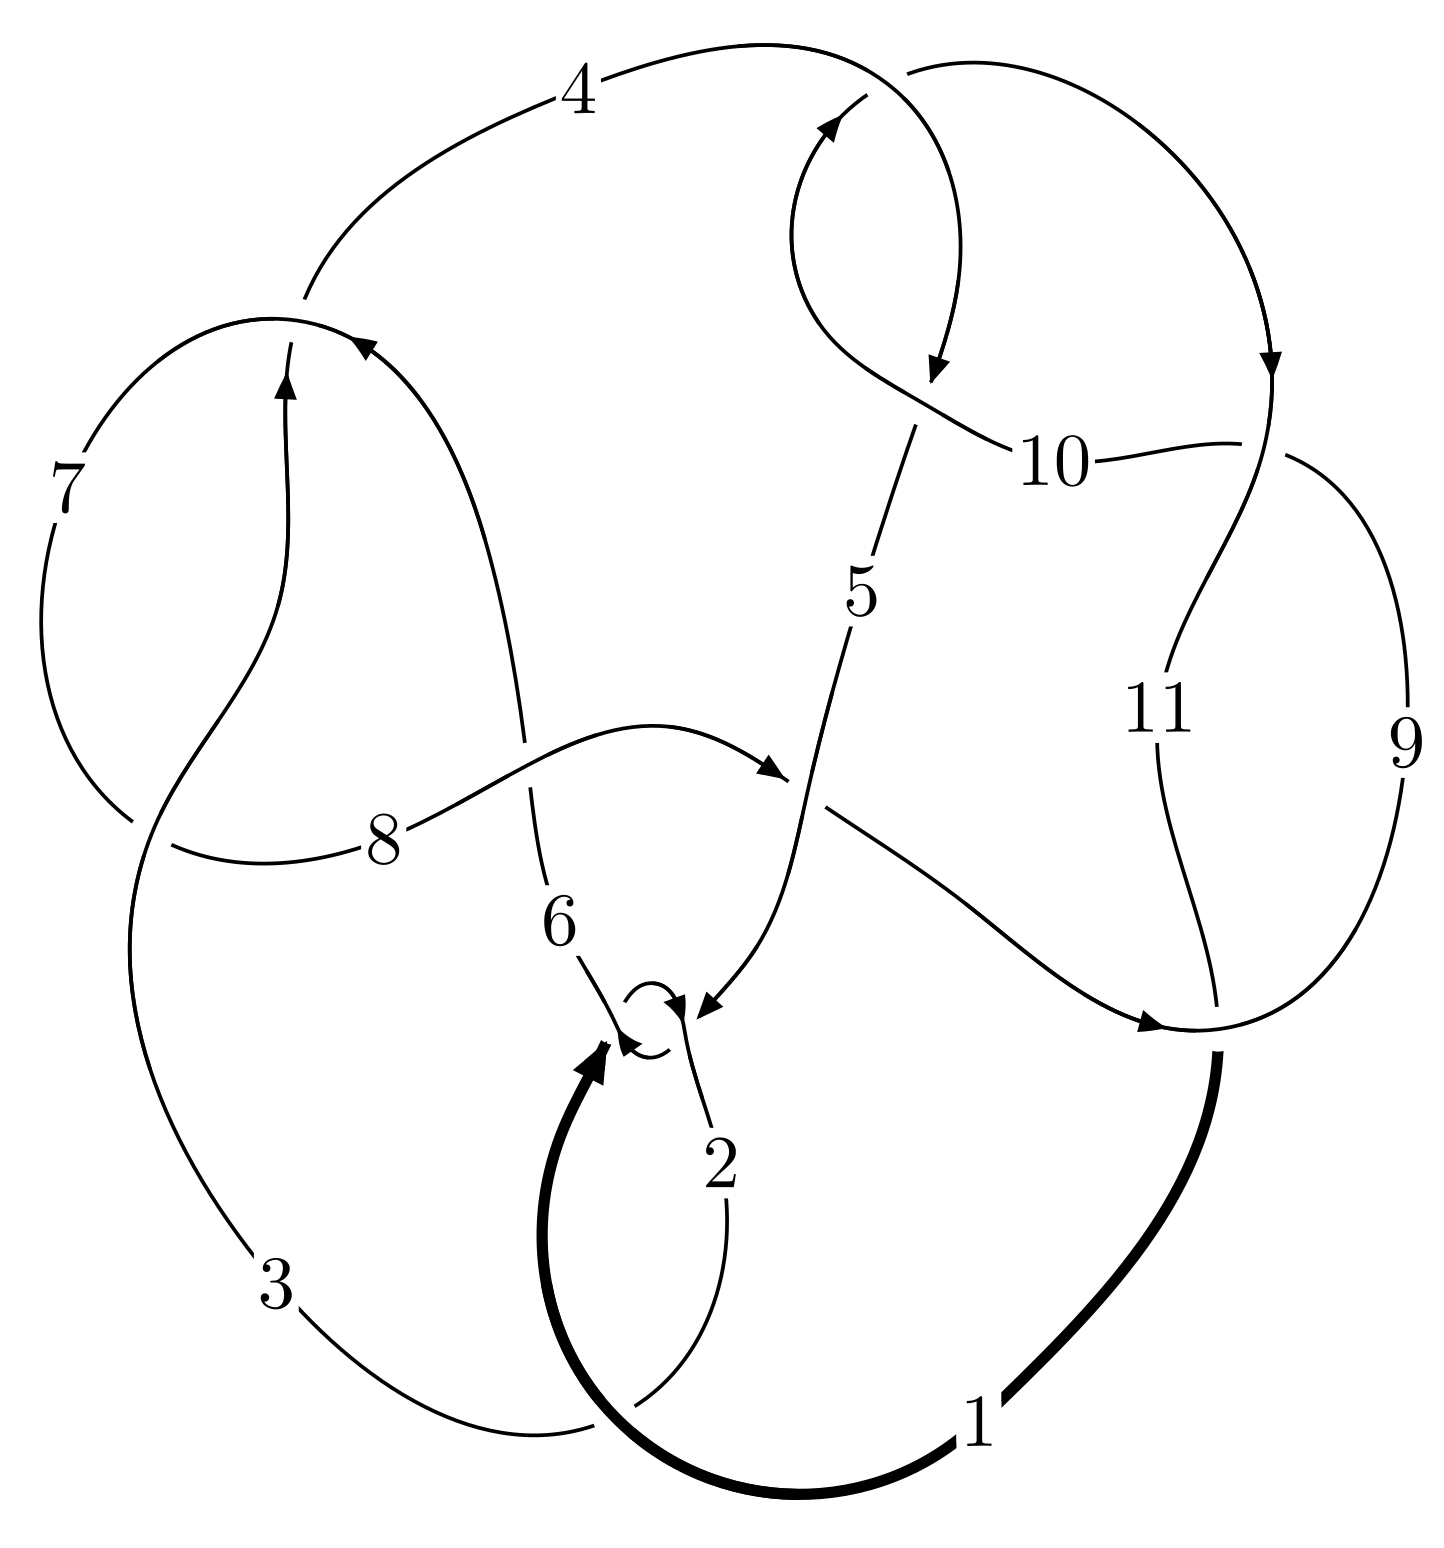
\includegraphics[width=112pt]{../../../GIT/diagram.site/Diagrams/png/377_11a_128.png}\\
\ \ \ A knot diagram\footnotemark}&
\allowdisplaybreaks
\textbf{Linearized knot diagam} \\
\cline{2-2}
 &
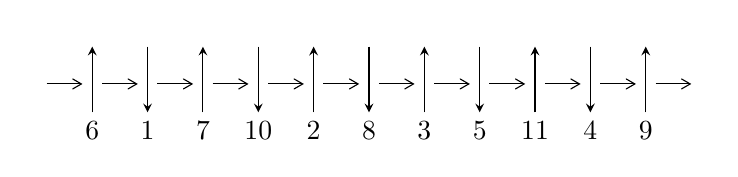
\begin{tikzpicture}[x=20pt, y=17pt]
	% nodes
	\node (C0) at (0, 0) {};
	\node (C1) at (1, 0) {};
	\node (C1U) at (1, +1) {};
	\node (C1D) at (1, -1) {6};

	\node (C2) at (2, 0) {};
	\node (C2U) at (2, +1) {};
	\node (C2D) at (2, -1) {1};

	\node (C3) at (3, 0) {};
	\node (C3U) at (3, +1) {};
	\node (C3D) at (3, -1) {7};

	\node (C4) at (4, 0) {};
	\node (C4U) at (4, +1) {};
	\node (C4D) at (4, -1) {10};

	\node (C5) at (5, 0) {};
	\node (C5U) at (5, +1) {};
	\node (C5D) at (5, -1) {2};

	\node (C6) at (6, 0) {};
	\node (C6U) at (6, +1) {};
	\node (C6D) at (6, -1) {8};

	\node (C7) at (7, 0) {};
	\node (C7U) at (7, +1) {};
	\node (C7D) at (7, -1) {3};

	\node (C8) at (8, 0) {};
	\node (C8U) at (8, +1) {};
	\node (C8D) at (8, -1) {5};

	\node (C9) at (9, 0) {};
	\node (C9U) at (9, +1) {};
	\node (C9D) at (9, -1) {11};

	\node (C10) at (10, 0) {};
	\node (C10U) at (10, +1) {};
	\node (C10D) at (10, -1) {4};

	\node (C11) at (11, 0) {};
	\node (C11U) at (11, +1) {};
	\node (C11D) at (11, -1) {9};
	\node (C12) at (12, 0) {};

	% arrows
	\draw[->,>={angle 60}]
	(C0) edge (C1) (C1) edge (C2) (C2) edge (C3) (C3) edge (C4) (C4) edge (C5) (C5) edge (C6) (C6) edge (C7) (C7) edge (C8) (C8) edge (C9) (C9) edge (C10) (C10) edge (C11) (C11) edge (C12) ;	\draw[->,>=stealth]
	(C1D) edge (C1U) (C2U) edge (C2D) (C3D) edge (C3U) (C4U) edge (C4D) (C5D) edge (C5U) (C6U) edge (C6D) (C7D) edge (C7U) (C8U) edge (C8D) (C9D) edge (C9U) (C10U) edge (C10D) (C11D) edge (C11U) ;
	\end{tikzpicture} \\
\hhline{~~} \\& 
\textbf{Solving Sequence} \\ \cline{2-2} 
 &
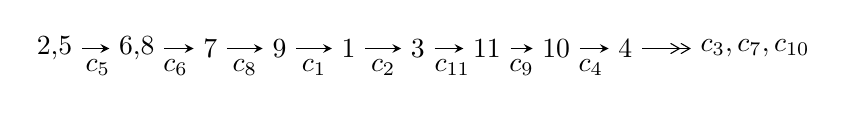
\begin{tikzpicture}[x=25pt, y=7pt]
	% node
	\node (A0) at (-1/8, 0) {2,5};
	\node (A1) at (17/16, 0) {6,8};
	\node (A2) at (17/8, 0) {7};
	\node (A3) at (25/8, 0) {9};
	\node (A4) at (33/8, 0) {1};
	\node (A5) at (41/8, 0) {3};
	\node (A6) at (49/8, 0) {11};
	\node (A7) at (57/8, 0) {10};
	\node (A8) at (65/8, 0) {4};
	\node (C1) at (1/2, -1) {$c_{5}$};
	\node (C2) at (13/8, -1) {$c_{6}$};
	\node (C3) at (21/8, -1) {$c_{8}$};
	\node (C4) at (29/8, -1) {$c_{1}$};
	\node (C5) at (37/8, -1) {$c_{2}$};
	\node (C6) at (45/8, -1) {$c_{11}$};
	\node (C7) at (53/8, -1) {$c_{9}$};
	\node (C8) at (61/8, -1) {$c_{4}$};
	\node (A9) at (10, 0) {$c_{3},c_{7},c_{10}$};

	% edge
	\draw[->,>=stealth]	
	(A0) edge (A1) (A1) edge (A2) (A2) edge (A3) (A3) edge (A4) (A4) edge (A5) (A5) edge (A6) (A6) edge (A7) (A7) edge (A8) ;
	\draw[->>,>={angle 60}]	
	(A8) edge (A9);
\end{tikzpicture} \\ 

\end{tabular} \\

\footnotetext{
The image of knot diagram is generated by the software ``\textbf{Draw programme}" developed by Andrew Bartholomew(\url{http://www.layer8.co.uk/maths/draw/index.htm\#Running-draw}), where we modified some parts for our purpose(\url{https://github.com/CATsTAILs/LinksPainter}).
}\phantom \\ \newline 
\centering \textbf{Ideals for irreducible components\footnotemark of $X_{\text{par}}$} 
 
\begin{align*}
I^u_{1}&=\langle 
- u^{27}+u^{26}+\cdots+8 b+1,\;- u^{27}+u^{26}+\cdots+8 a-7,\;u^{28}+6 u^{26}+\cdots-2 u+1\rangle \\
I^u_{2}&=\langle 
-1.55682\times10^{17} u^{41}+7.44166\times10^{16} u^{40}+\cdots+3.93707\times10^{17} b-4.00955\times10^{17},\\
\phantom{I^u_{2}}&\phantom{= \langle  }-3.62508\times10^{17} u^{41}+5.17336\times10^{17} u^{40}+\cdots+3.93707\times10^{17} a+8.90477\times10^{17},\;u^{42}- u^{41}+\cdots+2 u+1\rangle \\
I^u_{3}&=\langle 
b- a-1,\;a^3- a^2 u+3 a^2-2 a u+a-1,\;u^2+1\rangle \\
\\
\end{align*}
\raggedright * 3 irreducible components of $\dim_{\mathbb{C}}=0$, with total 76 representations.\\
\footnotetext{All coefficients of polynomials are rational numbers. But the coefficients are sometimes approximated in decimal forms when there is not enough margin.}
\newpage
\renewcommand{\arraystretch}{1}
\centering \section*{I. $I^u_{1}= \langle - u^{27}+u^{26}+\cdots+8 b+1,\;- u^{27}+u^{26}+\cdots+8 a-7,\;u^{28}+6 u^{26}+\cdots-2 u+1 \rangle$}
\flushleft \textbf{(i) Arc colorings}\\
\begin{tabular}{m{7pt} m{180pt} m{7pt} m{180pt} }
\flushright $a_{2}=$&$\begin{pmatrix}0\\u\end{pmatrix}$ \\
\flushright $a_{5}=$&$\begin{pmatrix}1\\0\end{pmatrix}$ \\
\flushright $a_{6}=$&$\begin{pmatrix}1\\- u^2\end{pmatrix}$ \\
\flushright $a_{8}=$&$\begin{pmatrix}\frac{1}{8} u^{27}-\frac{1}{8} u^{26}+\cdots+\frac{3}{8} u+\frac{7}{8}\\\frac{1}{8} u^{27}-\frac{1}{8} u^{26}+\cdots+\frac{3}{8} u-\frac{1}{8}\end{pmatrix}$ \\
\flushright $a_{7}=$&$\begin{pmatrix}\frac{1}{8} u^{27}-\frac{1}{8} u^{26}+\cdots+\frac{3}{8} u+\frac{7}{8}\\\frac{1}{8} u^{27}-\frac{1}{8} u^{26}+\cdots+\frac{3}{8} u-\frac{1}{8}\end{pmatrix}$ \\
\flushright $a_{9}=$&$\begin{pmatrix}u^4+u^2+1\\\frac{1}{8} u^{27}-\frac{1}{8} u^{26}+\cdots+\frac{3}{8} u-\frac{1}{8}\end{pmatrix}$ \\
\flushright $a_{1}=$&$\begin{pmatrix}- u\\u^3+u\end{pmatrix}$ \\
\flushright $a_{3}=$&$\begin{pmatrix}- u^3\\u^5+u^3+u\end{pmatrix}$ \\
\flushright $a_{11}=$&$\begin{pmatrix}\frac{1}{8} u^{27}+\frac{1}{8} u^{26}+\cdots-\frac{17}{8} u+\frac{1}{8}\\\frac{5}{8} u^{27}+\frac{7}{8} u^{26}+\cdots-\frac{3}{8} u+\frac{9}{8}\end{pmatrix}$ \\
\flushright $a_{10}=$&$\begin{pmatrix}-\frac{3}{4} u^{27}+\frac{1}{4} u^{26}+\cdots-2 u+\frac{3}{2}\\-\frac{9}{8} u^{27}-\frac{5}{8} u^{26}+\cdots-\frac{19}{8} u-\frac{1}{8}\end{pmatrix}$ \\
\flushright $a_{4}=$&$\begin{pmatrix}-\frac{1}{8} u^{27}-\frac{1}{8} u^{26}+\cdots+\frac{9}{8} u-\frac{1}{8}\\-\frac{1}{8} u^{27}-\frac{1}{8} u^{26}+\cdots+\frac{9}{8} u-\frac{1}{8}\end{pmatrix}$\\ \flushright $a_{4}=$&$\begin{pmatrix}-\frac{1}{8} u^{27}-\frac{1}{8} u^{26}+\cdots+\frac{9}{8} u-\frac{1}{8}\\-\frac{1}{8} u^{27}-\frac{1}{8} u^{26}+\cdots+\frac{9}{8} u-\frac{1}{8}\end{pmatrix}$\\&\end{tabular}
\flushleft \textbf{(ii) Obstruction class $= -1$}\\~\\
\flushleft \textbf{(iii) Cusp Shapes $= -\frac{9}{2} u^{27}-26 u^{25}+\cdots-20 u+\frac{7}{2}$}\\~\\
\newpage\renewcommand{\arraystretch}{1}
\flushleft \textbf{(iv) u-Polynomials at the component}\newline \\
\begin{tabular}{m{50pt}|m{274pt}}
Crossings & \hspace{64pt}u-Polynomials at each crossing \\
\hline $$\begin{aligned}c_{1},c_{3},c_{5}\\c_{7}\end{aligned}$$&$\begin{aligned}
&u^{28}+6 u^{26}+\cdots-2 u+1
\end{aligned}$\\
\hline $$\begin{aligned}c_{2},c_{6}\end{aligned}$$&$\begin{aligned}
&u^{28}+12 u^{27}+\cdots+10 u+1
\end{aligned}$\\
\hline $$\begin{aligned}c_{4},c_{10}\end{aligned}$$&$\begin{aligned}
&u^{28}+3 u^{27}+\cdots+u+2
\end{aligned}$\\
\hline $$\begin{aligned}c_{8}\end{aligned}$$&$\begin{aligned}
&u^{28}-15 u^{27}+\cdots-785 u+86
\end{aligned}$\\
\hline $$\begin{aligned}c_{9},c_{11}\end{aligned}$$&$\begin{aligned}
&u^{28}-9 u^{27}+\cdots-19 u+4
\end{aligned}$\\
\hline
\end{tabular}\\~\\
\newpage\renewcommand{\arraystretch}{1}
\flushleft \textbf{(v) Riley Polynomials at the component}\newline \\
\begin{tabular}{m{50pt}|m{274pt}}
Crossings & \hspace{64pt}Riley Polynomials at each crossing \\
\hline $$\begin{aligned}c_{1},c_{3},c_{5}\\c_{7}\end{aligned}$$&$\begin{aligned}
&y^{28}+12 y^{27}+\cdots+10 y+1
\end{aligned}$\\
\hline $$\begin{aligned}c_{2},c_{6}\end{aligned}$$&$\begin{aligned}
&y^{28}+16 y^{27}+\cdots+30 y+1
\end{aligned}$\\
\hline $$\begin{aligned}c_{4},c_{10}\end{aligned}$$&$\begin{aligned}
&y^{28}+9 y^{27}+\cdots+19 y+4
\end{aligned}$\\
\hline $$\begin{aligned}c_{8}\end{aligned}$$&$\begin{aligned}
&y^{28}-3 y^{27}+\cdots+53715 y+7396
\end{aligned}$\\
\hline $$\begin{aligned}c_{9},c_{11}\end{aligned}$$&$\begin{aligned}
&y^{28}+21 y^{27}+\cdots+111 y+16
\end{aligned}$\\
\hline
\end{tabular}\\~\\
\newpage\flushleft \textbf{(vi) Complex Volumes and Cusp Shapes}
$$\begin{array}{c|c|c}  
\text{Solutions to }I^u_{1}& \I (\text{vol} + \sqrt{-1}CS) & \text{Cusp shape}\\
 \hline 
\begin{aligned}
u &= -0.759562 + 0.603461 I \\
a &= \phantom{-}0.262237 - 0.123439 I \\
b &= -0.155404 + 1.183400 I\end{aligned}
 & \phantom{-}5.48513 - 0.99092 I & \phantom{-}8.59434 + 2.33645 I \\ \hline\begin{aligned}
u &= -0.759562 - 0.603461 I \\
a &= \phantom{-}0.262237 + 0.123439 I \\
b &= -0.155404 - 1.183400 I\end{aligned}
 & \phantom{-}5.48513 + 0.99092 I & \phantom{-}8.59434 - 2.33645 I \\ \hline\begin{aligned}
u &= \phantom{-}0.616775 + 0.724242 I \\
a &= -0.025809 - 0.273919 I \\
b &= -0.104321 - 0.909807 I\end{aligned}
 & \phantom{-}0.69719 + 2.24985 I & \phantom{-}1.09419 - 3.47682 I \\ \hline\begin{aligned}
u &= \phantom{-}0.616775 - 0.724242 I \\
a &= -0.025809 + 0.273919 I \\
b &= -0.104321 + 0.909807 I\end{aligned}
 & \phantom{-}0.69719 - 2.24985 I & \phantom{-}1.09419 + 3.47682 I \\ \hline\begin{aligned}
u &= -0.724810 + 0.770942 I \\
a &= -0.188930 - 0.061129 I \\
b &= \phantom{-}0.124282 + 0.902212 I\end{aligned}
 & \phantom{-}2.05272 - 7.06945 I & \phantom{-}3.67598 + 8.34686 I \\ \hline\begin{aligned}
u &= -0.724810 - 0.770942 I \\
a &= -0.188930 + 0.061129 I \\
b &= \phantom{-}0.124282 - 0.902212 I\end{aligned}
 & \phantom{-}2.05272 + 7.06945 I & \phantom{-}3.67598 - 8.34686 I \\ \hline\begin{aligned}
u &= -0.802758 + 0.434476 I \\
a &= \phantom{-}0.573015 - 0.162109 I \\
b &= -0.603664 + 1.171140 I\end{aligned}
 & \phantom{-}1.06471 + 4.87874 I & \phantom{-}4.05798 - 2.77982 I \\ \hline\begin{aligned}
u &= -0.802758 - 0.434476 I \\
a &= \phantom{-}0.573015 + 0.162109 I \\
b &= -0.603664 - 1.171140 I\end{aligned}
 & \phantom{-}1.06471 - 4.87874 I & \phantom{-}4.05798 + 2.77982 I \\ \hline\begin{aligned}
u &= \phantom{-}0.416029 + 1.025630 I \\
a &= -1.55269 - 1.44392 I \\
b &= -1.71795 - 0.79732 I\end{aligned}
 & -6.63635 - 0.10967 I & -3.90050 - 2.81899 I \\ \hline\begin{aligned}
u &= \phantom{-}0.416029 - 1.025630 I \\
a &= -1.55269 + 1.44392 I \\
b &= -1.71795 + 0.79732 I\end{aligned}
 & -6.63635 + 0.10967 I & -3.90050 + 2.81899 I\\
 \hline 
 \end{array}$$\newpage$$\begin{array}{c|c|c}  
\text{Solutions to }I^u_{1}& \I (\text{vol} + \sqrt{-1}CS) & \text{Cusp shape}\\
 \hline 
\begin{aligned}
u &= -0.436495 + 1.052560 I \\
a &= -1.72314 + 1.24024 I \\
b &= -1.80300 + 0.47325 I\end{aligned}
 & -7.02411 - 5.90283 I & -4.75289 + 7.68964 I \\ \hline\begin{aligned}
u &= -0.436495 - 1.052560 I \\
a &= -1.72314 - 1.24024 I \\
b &= -1.80300 - 0.47325 I\end{aligned}
 & -7.02411 + 5.90283 I & -4.75289 - 7.68964 I \\ \hline\begin{aligned}
u &= \phantom{-}0.606810 + 1.011990 I \\
a &= -1.232890 - 0.281742 I \\
b &= -0.498787 + 0.101237 I\end{aligned}
 & \phantom{-}0.54803 + 3.32331 I & \phantom{-}2.18088 - 2.29510 I \\ \hline\begin{aligned}
u &= \phantom{-}0.606810 - 1.011990 I \\
a &= -1.232890 + 0.281742 I \\
b &= -0.498787 - 0.101237 I\end{aligned}
 & \phantom{-}0.54803 - 3.32331 I & \phantom{-}2.18088 + 2.29510 I \\ \hline\begin{aligned}
u &= \phantom{-}0.715634 + 0.398949 I \\
a &= \phantom{-}0.607712 + 0.041457 I \\
b &= -0.543805 - 0.932641 I\end{aligned}
 & \phantom{-}0.030119 + 0.482942 I & \phantom{-}2.45869 - 2.54239 I \\ \hline\begin{aligned}
u &= \phantom{-}0.715634 - 0.398949 I \\
a &= \phantom{-}0.607712 - 0.041457 I \\
b &= -0.543805 + 0.932641 I\end{aligned}
 & \phantom{-}0.030119 - 0.482942 I & \phantom{-}2.45869 + 2.54239 I \\ \hline\begin{aligned}
u &= -0.570794 + 1.089040 I \\
a &= -1.68154 + 0.34539 I \\
b &= -1.015660 - 0.550205 I\end{aligned}
 & -1.89491 - 7.14346 I & -3.37367 + 6.75053 I \\ \hline\begin{aligned}
u &= -0.570794 - 1.089040 I \\
a &= -1.68154 - 0.34539 I \\
b &= -1.015660 + 0.550205 I\end{aligned}
 & -1.89491 + 7.14346 I & -3.37367 - 6.75053 I \\ \hline\begin{aligned}
u &= \phantom{-}0.626024 + 1.122830 I \\
a &= -1.73728 - 0.00452 I \\
b &= -0.646939 + 1.032570 I\end{aligned}
 & \phantom{-}2.17277 + 9.75277 I & \phantom{-}3.46320 - 8.11852 I \\ \hline\begin{aligned}
u &= \phantom{-}0.626024 - 1.122830 I \\
a &= -1.73728 + 0.00452 I \\
b &= -0.646939 - 1.032570 I\end{aligned}
 & \phantom{-}2.17277 - 9.75277 I & \phantom{-}3.46320 + 8.11852 I\\
 \hline 
 \end{array}$$\newpage$$\begin{array}{c|c|c}  
\text{Solutions to }I^u_{1}& \I (\text{vol} + \sqrt{-1}CS) & \text{Cusp shape}\\
 \hline 
\begin{aligned}
u &= \phantom{-}0.023188 + 0.692895 I \\
a &= \phantom{-}2.34879 - 0.20424 I \\
b &= \phantom{-}1.59940 - 0.20555 I\end{aligned}
 & -4.98395 + 2.93184 I & \phantom{-}0.79314 - 3.40006 I \\ \hline\begin{aligned}
u &= \phantom{-}0.023188 - 0.692895 I \\
a &= \phantom{-}2.34879 + 0.20424 I \\
b &= \phantom{-}1.59940 + 0.20555 I\end{aligned}
 & -4.98395 - 2.93184 I & \phantom{-}0.79314 + 3.40006 I \\ \hline\begin{aligned}
u &= -0.588545 + 1.173310 I \\
a &= -2.06199 + 0.06635 I \\
b &= -1.18576 - 1.39834 I\end{aligned}
 & -4.61324 - 9.81937 I & -3.57047 + 5.81179 I \\ \hline\begin{aligned}
u &= -0.588545 - 1.173310 I \\
a &= -2.06199 - 0.06635 I \\
b &= -1.18576 + 1.39834 I\end{aligned}
 & -4.61324 + 9.81937 I & -3.57047 - 5.81179 I \\ \hline\begin{aligned}
u &= \phantom{-}0.605210 + 1.183850 I \\
a &= -2.06950 + 0.03808 I \\
b &= -1.05260 + 1.57196 I\end{aligned}
 & -3.5733 + 15.6943 I & -1.82098 - 10.41623 I \\ \hline\begin{aligned}
u &= \phantom{-}0.605210 - 1.183850 I \\
a &= -2.06950 - 0.03808 I \\
b &= -1.05260 - 1.57196 I\end{aligned}
 & -3.5733 - 15.6943 I & -1.82098 + 10.41623 I \\ \hline\begin{aligned}
u &= \phantom{-}0.273295 + 0.395938 I \\
a &= \phantom{-}0.982020 - 0.270229 I \\
b &= \phantom{-}0.104195 - 0.451120 I\end{aligned}
 & \phantom{-}0.225861 + 1.065080 I & \phantom{-}3.10010 - 6.65254 I \\ \hline\begin{aligned}
u &= \phantom{-}0.273295 - 0.395938 I \\
a &= \phantom{-}0.982020 + 0.270229 I \\
b &= \phantom{-}0.104195 + 0.451120 I\end{aligned}
 & \phantom{-}0.225861 - 1.065080 I & \phantom{-}3.10010 + 6.65254 I\\
 \hline 
 \end{array}$$\newpage\newpage\renewcommand{\arraystretch}{1}
\centering \section*{II. $I^u_{2}= \langle -1.56\times10^{17} u^{41}+7.44\times10^{16} u^{40}+\cdots+3.94\times10^{17} b-4.01\times10^{17},\;-3.63\times10^{17} u^{41}+5.17\times10^{17} u^{40}+\cdots+3.94\times10^{17} a+8.90\times10^{17},\;u^{42}- u^{41}+\cdots+2 u+1 \rangle$}
\flushleft \textbf{(i) Arc colorings}\\
\begin{tabular}{m{7pt} m{180pt} m{7pt} m{180pt} }
\flushright $a_{2}=$&$\begin{pmatrix}0\\u\end{pmatrix}$ \\
\flushright $a_{5}=$&$\begin{pmatrix}1\\0\end{pmatrix}$ \\
\flushright $a_{6}=$&$\begin{pmatrix}1\\- u^2\end{pmatrix}$ \\
\flushright $a_{8}=$&$\begin{pmatrix}0.920756 u^{41}-1.31402 u^{40}+\cdots-0.678222 u-2.26178\\0.395427 u^{41}-0.189015 u^{40}+\cdots+0.318945 u+1.01841\end{pmatrix}$ \\
\flushright $a_{7}=$&$\begin{pmatrix}0.525329 u^{41}-1.12500 u^{40}+\cdots-0.997167 u-2.28019\\0.154289 u^{41}-0.155024 u^{40}+\cdots+0.0143489 u+1.24208\end{pmatrix}$ \\
\flushright $a_{9}=$&$\begin{pmatrix}0.525329 u^{41}-1.12500 u^{40}+\cdots-0.997167 u-3.28019\\0.395427 u^{41}-0.189015 u^{40}+\cdots+0.318945 u+1.01841\end{pmatrix}$ \\
\flushright $a_{1}=$&$\begin{pmatrix}- u\\u^3+u\end{pmatrix}$ \\
\flushright $a_{3}=$&$\begin{pmatrix}- u^3\\u^5+u^3+u\end{pmatrix}$ \\
\flushright $a_{11}=$&$\begin{pmatrix}-1.16179 u^{41}+1.49863 u^{40}+\cdots-7.64525 u-3.07967\\-0.0610512 u^{41}+0.300717 u^{40}+\cdots+4.24243 u+0.892006\end{pmatrix}$ \\
\flushright $a_{10}=$&$\begin{pmatrix}-1.05647 u^{41}-0.115032 u^{40}+\cdots+1.79735 u+2.62565\\0.333742 u^{41}-0.317542 u^{40}+\cdots-2.13420 u-1.49818\end{pmatrix}$ \\
\flushright $a_{4}=$&$\begin{pmatrix}1.61808 u^{41}-1.69040 u^{40}+\cdots+4.35493 u+2.24321\\-0.222935 u^{41}+0.0950704 u^{40}+\cdots-2.85741 u-0.597649\end{pmatrix}$\\ \flushright $a_{4}=$&$\begin{pmatrix}1.61808 u^{41}-1.69040 u^{40}+\cdots+4.35493 u+2.24321\\-0.222935 u^{41}+0.0950704 u^{40}+\cdots-2.85741 u-0.597649\end{pmatrix}$\\&\end{tabular}
\flushleft \textbf{(ii) Obstruction class $= -1$}\\~\\
\flushleft \textbf{(iii) Cusp Shapes $= -\frac{750018447371229972}{393706681309071797} u^{41}+\frac{1326377308854531456}{393706681309071797} u^{40}+\cdots+\frac{3939201724436401700}{393706681309071797} u+\frac{974136661643821530}{393706681309071797}$}\\~\\
\newpage\renewcommand{\arraystretch}{1}
\flushleft \textbf{(iv) u-Polynomials at the component}\newline \\
\begin{tabular}{m{50pt}|m{274pt}}
Crossings & \hspace{64pt}u-Polynomials at each crossing \\
\hline $$\begin{aligned}c_{1},c_{3},c_{5}\\c_{7}\end{aligned}$$&$\begin{aligned}
&u^{42}- u^{41}+\cdots+2 u+1
\end{aligned}$\\
\hline $$\begin{aligned}c_{2},c_{6}\end{aligned}$$&$\begin{aligned}
&u^{42}+23 u^{41}+\cdots+22 u^2+1
\end{aligned}$\\
\hline $$\begin{aligned}c_{4},c_{10}\end{aligned}$$&$\begin{aligned}
&(u^{21}- u^{20}+\cdots+u-1)^{2}
\end{aligned}$\\
\hline $$\begin{aligned}c_{8}\end{aligned}$$&$\begin{aligned}
&(u^{21}+5 u^{20}+\cdots-11 u-3)^{2}
\end{aligned}$\\
\hline $$\begin{aligned}c_{9},c_{11}\end{aligned}$$&$\begin{aligned}
&(u^{21}-7 u^{20}+\cdots+3 u+1)^{2}
\end{aligned}$\\
\hline
\end{tabular}\\~\\
\newpage\renewcommand{\arraystretch}{1}
\flushleft \textbf{(v) Riley Polynomials at the component}\newline \\
\begin{tabular}{m{50pt}|m{274pt}}
Crossings & \hspace{64pt}Riley Polynomials at each crossing \\
\hline $$\begin{aligned}c_{1},c_{3},c_{5}\\c_{7}\end{aligned}$$&$\begin{aligned}
&y^{42}+23 y^{41}+\cdots+22 y^2+1
\end{aligned}$\\
\hline $$\begin{aligned}c_{2},c_{6}\end{aligned}$$&$\begin{aligned}
&y^{42}-9 y^{41}+\cdots+44 y+1
\end{aligned}$\\
\hline $$\begin{aligned}c_{4},c_{10}\end{aligned}$$&$\begin{aligned}
&(y^{21}+7 y^{20}+\cdots+3 y-1)^{2}
\end{aligned}$\\
\hline $$\begin{aligned}c_{8}\end{aligned}$$&$\begin{aligned}
&(y^{21}+3 y^{20}+\cdots-41 y-9)^{2}
\end{aligned}$\\
\hline $$\begin{aligned}c_{9},c_{11}\end{aligned}$$&$\begin{aligned}
&(y^{21}+15 y^{20}+\cdots+27 y-1)^{2}
\end{aligned}$\\
\hline
\end{tabular}\\~\\
\newpage\flushleft \textbf{(vi) Complex Volumes and Cusp Shapes}
$$\begin{array}{c|c|c}  
\text{Solutions to }I^u_{2}& \I (\text{vol} + \sqrt{-1}CS) & \text{Cusp shape}\\
 \hline 
\begin{aligned}
u &= \phantom{-}0.384983 + 0.893506 I \\
a &= -1.61437 - 0.96323 I \\
b &= -0.207726 + 0.818105 I\end{aligned}
 & -1.26832 + 1.59690 I & \phantom{-}3.13274 - 4.73829 I \\ \hline\begin{aligned}
u &= \phantom{-}0.384983 - 0.893506 I \\
a &= -1.61437 + 0.96323 I \\
b &= -0.207726 - 0.818105 I\end{aligned}
 & -1.26832 - 1.59690 I & \phantom{-}3.13274 + 4.73829 I \\ \hline\begin{aligned}
u &= \phantom{-}0.900670 + 0.302277 I \\
a &= -0.0782845 - 0.0466257 I \\
b &= \phantom{-}0.86562 + 1.42640 I\end{aligned}
 & -0.91901 - 10.18330 I & \phantom{-}1.25382 + 7.21296 I \\ \hline\begin{aligned}
u &= \phantom{-}0.900670 - 0.302277 I \\
a &= -0.0782845 + 0.0466257 I \\
b &= \phantom{-}0.86562 - 1.42640 I\end{aligned}
 & -0.91901 + 10.18330 I & \phantom{-}1.25382 - 7.21296 I \\ \hline\begin{aligned}
u &= -0.656782 + 0.830369 I \\
a &= \phantom{-}1.211820 - 0.034605 I \\
b &= \phantom{-}0.128800 + 0.461641 I\end{aligned}
 & \phantom{-}1.85425 + 1.80763 I & \phantom{-}4.25907 - 2.73625 I \\ \hline\begin{aligned}
u &= -0.656782 - 0.830369 I \\
a &= \phantom{-}1.211820 + 0.034605 I \\
b &= \phantom{-}0.128800 - 0.461641 I\end{aligned}
 & \phantom{-}1.85425 - 1.80763 I & \phantom{-}4.25907 + 2.73625 I \\ \hline\begin{aligned}
u &= \phantom{-}0.843980 + 0.412000 I \\
a &= \phantom{-}0.264230 - 0.021493 I \\
b &= \phantom{-}0.433674 + 1.104090 I\end{aligned}
 & \phantom{-}4.29768 - 4.29720 I & \phantom{-}6.75143 + 3.93304 I \\ \hline\begin{aligned}
u &= \phantom{-}0.843980 - 0.412000 I \\
a &= \phantom{-}0.264230 + 0.021493 I \\
b &= \phantom{-}0.433674 - 1.104090 I\end{aligned}
 & \phantom{-}4.29768 + 4.29720 I & \phantom{-}6.75143 - 3.93304 I \\ \hline\begin{aligned}
u &= \phantom{-}0.742093 + 0.573520 I \\
a &= \phantom{-}0.729163 + 0.038018 I \\
b &= \phantom{-}0.128800 + 0.461641 I\end{aligned}
 & \phantom{-}1.85425 + 1.80763 I & \phantom{-}4.25907 - 2.73625 I \\ \hline\begin{aligned}
u &= \phantom{-}0.742093 - 0.573520 I \\
a &= \phantom{-}0.729163 - 0.038018 I \\
b &= \phantom{-}0.128800 - 0.461641 I\end{aligned}
 & \phantom{-}1.85425 - 1.80763 I & \phantom{-}4.25907 + 2.73625 I\\
 \hline 
 \end{array}$$\newpage$$\begin{array}{c|c|c}  
\text{Solutions to }I^u_{2}& \I (\text{vol} + \sqrt{-1}CS) & \text{Cusp shape}\\
 \hline 
\begin{aligned}
u &= \phantom{-}0.528906 + 0.927109 I \\
a &= \phantom{-}1.321410 + 0.194864 I \\
b &= \phantom{-}0.641247 - 0.630310 I\end{aligned}
 & \phantom{-}0.10785 + 2.26276 I & -0.12423 - 3.11409 I \\ \hline\begin{aligned}
u &= \phantom{-}0.528906 - 0.927109 I \\
a &= \phantom{-}1.321410 - 0.194864 I \\
b &= \phantom{-}0.641247 + 0.630310 I\end{aligned}
 & \phantom{-}0.10785 - 2.26276 I & -0.12423 + 3.11409 I \\ \hline\begin{aligned}
u &= -0.860486 + 0.285796 I \\
a &= -0.0772165 - 0.0782315 I \\
b &= \phantom{-}0.93790 - 1.24922 I\end{aligned}
 & -1.96895 + 4.48385 I & -0.56586 - 2.47352 I \\ \hline\begin{aligned}
u &= -0.860486 - 0.285796 I \\
a &= -0.0772165 + 0.0782315 I \\
b &= \phantom{-}0.93790 + 1.24922 I\end{aligned}
 & -1.96895 - 4.48385 I & -0.56586 + 2.47352 I \\ \hline\begin{aligned}
u &= -0.239332 + 1.082520 I \\
a &= -1.021360 + 0.939730 I \\
b &= -0.510732\phantom{ +0.000000I}\end{aligned}
 & -4.11368\phantom{ +0.000000I} & -8.21539 + 0. I\phantom{ +0.000000I} \\ \hline\begin{aligned}
u &= -0.239332 - 1.082520 I \\
a &= -1.021360 - 0.939730 I \\
b &= -0.510732\phantom{ +0.000000I}\end{aligned}
 & -4.11368\phantom{ +0.000000I} & -8.21539 + 0. I\phantom{ +0.000000I} \\ \hline\begin{aligned}
u &= \phantom{-}0.125880 + 1.108300 I \\
a &= \phantom{-}0.910717 + 0.374635 I \\
b &= \phantom{-}1.127110 + 0.099375 I\end{aligned}
 & -4.65974 + 2.68588 I & -1.85070 - 3.67518 I \\ \hline\begin{aligned}
u &= \phantom{-}0.125880 - 1.108300 I \\
a &= \phantom{-}0.910717 - 0.374635 I \\
b &= \phantom{-}1.127110 - 0.099375 I\end{aligned}
 & -4.65974 - 2.68588 I & -1.85070 + 3.67518 I \\ \hline\begin{aligned}
u &= \phantom{-}0.478722 + 1.037960 I \\
a &= -1.54549 - 1.29421 I \\
b &= -0.98839 + 1.06606 I\end{aligned}
 & -6.19421 + 6.51836 I & -3.49661 - 6.69162 I \\ \hline\begin{aligned}
u &= \phantom{-}0.478722 - 1.037960 I \\
a &= -1.54549 + 1.29421 I \\
b &= -0.98839 - 1.06606 I\end{aligned}
 & -6.19421 - 6.51836 I & -3.49661 + 6.69162 I\\
 \hline 
 \end{array}$$\newpage$$\begin{array}{c|c|c}  
\text{Solutions to }I^u_{2}& \I (\text{vol} + \sqrt{-1}CS) & \text{Cusp shape}\\
 \hline 
\begin{aligned}
u &= -0.444142 + 1.066230 I \\
a &= -1.44535 + 1.30052 I \\
b &= -1.065450 - 0.815532 I\end{aligned}
 & -6.94955 - 0.90110 I & -5.44354 + 1.25880 I \\ \hline\begin{aligned}
u &= -0.444142 - 1.066230 I \\
a &= -1.44535 - 1.30052 I \\
b &= -1.065450 + 0.815532 I\end{aligned}
 & -6.94955 + 0.90110 I & -5.44354 - 1.25880 I \\ \hline\begin{aligned}
u &= -0.638288 + 0.999696 I \\
a &= \phantom{-}1.45241 - 0.09124 I \\
b &= \phantom{-}0.433674 + 1.104090 I\end{aligned}
 & \phantom{-}4.29768 - 4.29720 I & \phantom{-}6.75143 + 3.93304 I \\ \hline\begin{aligned}
u &= -0.638288 - 0.999696 I \\
a &= \phantom{-}1.45241 + 0.09124 I \\
b &= \phantom{-}0.433674 - 1.104090 I\end{aligned}
 & \phantom{-}4.29768 + 4.29720 I & \phantom{-}6.75143 - 3.93304 I \\ \hline\begin{aligned}
u &= -0.046915 + 1.192480 I \\
a &= \phantom{-}0.505321 - 0.535434 I \\
b &= \phantom{-}0.882596 - 0.417746 I\end{aligned}
 & -4.44976 + 2.73152 I & -0.80842 - 2.00184 I \\ \hline\begin{aligned}
u &= -0.046915 - 1.192480 I \\
a &= \phantom{-}0.505321 + 0.535434 I \\
b &= \phantom{-}0.882596 + 0.417746 I\end{aligned}
 & -4.44976 - 2.73152 I & -0.80842 + 2.00184 I \\ \hline\begin{aligned}
u &= -0.690143 + 0.400372 I \\
a &= \phantom{-}0.429900 - 0.357030 I \\
b &= \phantom{-}0.641247 - 0.630310 I\end{aligned}
 & \phantom{-}0.10785 + 2.26276 I & -0.12423 - 3.11409 I \\ \hline\begin{aligned}
u &= -0.690143 - 0.400372 I \\
a &= \phantom{-}0.429900 + 0.357030 I \\
b &= \phantom{-}0.641247 + 0.630310 I\end{aligned}
 & \phantom{-}0.10785 - 2.26276 I & -0.12423 + 3.11409 I \\ \hline\begin{aligned}
u &= \phantom{-}0.580018 + 1.088560 I \\
a &= \phantom{-}1.53519 + 0.23279 I \\
b &= \phantom{-}0.93790 - 1.24922 I\end{aligned}
 & -1.96895 + 4.48385 I & -0.56586 - 2.47352 I \\ \hline\begin{aligned}
u &= \phantom{-}0.580018 - 1.088560 I \\
a &= \phantom{-}1.53519 - 0.23279 I \\
b &= \phantom{-}0.93790 + 1.24922 I\end{aligned}
 & -1.96895 - 4.48385 I & -0.56586 + 2.47352 I\\
 \hline 
 \end{array}$$\newpage$$\begin{array}{c|c|c}  
\text{Solutions to }I^u_{2}& \I (\text{vol} + \sqrt{-1}CS) & \text{Cusp shape}\\
 \hline 
\begin{aligned}
u &= \phantom{-}0.135211 + 1.234020 I \\
a &= -0.331836 - 1.074640 I \\
b &= -0.207726 - 0.818105 I\end{aligned}
 & -1.26832 - 1.59690 I & \phantom{-}3.13274 + 4.73829 I \\ \hline\begin{aligned}
u &= \phantom{-}0.135211 - 1.234020 I \\
a &= -0.331836 + 1.074640 I \\
b &= -0.207726 + 0.818105 I\end{aligned}
 & -1.26832 + 1.59690 I & \phantom{-}3.13274 - 4.73829 I \\ \hline\begin{aligned}
u &= -0.613478 + 1.100460 I \\
a &= \phantom{-}1.58130 - 0.19672 I \\
b &= \phantom{-}0.86562 + 1.42640 I\end{aligned}
 & -0.91901 - 10.18330 I & \phantom{-}1.00000 + 7.21296 I \\ \hline\begin{aligned}
u &= -0.613478 - 1.100460 I \\
a &= \phantom{-}1.58130 + 0.19672 I \\
b &= \phantom{-}0.86562 - 1.42640 I\end{aligned}
 & -0.91901 + 10.18330 I & \phantom{-}1.00000 - 7.21296 I \\ \hline\begin{aligned}
u &= -0.264739 + 1.262700 I \\
a &= -0.67780 + 1.45363 I \\
b &= -1.065450 + 0.815532 I\end{aligned}
 & -6.94955 + 0.90110 I & -5.44354 - 1.25880 I \\ \hline\begin{aligned}
u &= -0.264739 - 1.262700 I \\
a &= -0.67780 - 1.45363 I \\
b &= -1.065450 - 0.815532 I\end{aligned}
 & -6.94955 - 0.90110 I & -5.44354 + 1.25880 I \\ \hline\begin{aligned}
u &= \phantom{-}0.243106 + 1.291400 I \\
a &= -0.55702 - 1.49792 I \\
b &= -0.98839 - 1.06606 I\end{aligned}
 & -6.19421 - 6.51836 I & -3.49661 + 6.69162 I \\ \hline\begin{aligned}
u &= \phantom{-}0.243106 - 1.291400 I \\
a &= -0.55702 + 1.49792 I \\
b &= -0.98839 + 1.06606 I\end{aligned}
 & -6.19421 + 6.51836 I & -3.49661 - 6.69162 I \\ \hline\begin{aligned}
u &= \phantom{-}0.315798 + 0.452715 I \\
a &= -2.24033 - 1.05440 I \\
b &= \phantom{-}0.882596 + 0.417746 I\end{aligned}
 & -4.44976 - 2.73152 I & -0.80842 + 2.00184 I \\ \hline\begin{aligned}
u &= \phantom{-}0.315798 - 0.452715 I \\
a &= -2.24033 + 1.05440 I \\
b &= \phantom{-}0.882596 - 0.417746 I\end{aligned}
 & -4.44976 + 2.73152 I & -0.80842 - 2.00184 I\\
 \hline 
 \end{array}$$\newpage$$\begin{array}{c|c|c}  
\text{Solutions to }I^u_{2}& \I (\text{vol} + \sqrt{-1}CS) & \text{Cusp shape}\\
 \hline 
\begin{aligned}
u &= -0.325064 + 0.154969 I \\
a &= -1.85243 + 2.34864 I \\
b &= \phantom{-}1.127110 - 0.099375 I\end{aligned}
 & -4.65974 - 2.68588 I & -1.85070 + 3.67518 I \\ \hline\begin{aligned}
u &= -0.325064 - 0.154969 I \\
a &= -1.85243 - 2.34864 I \\
b &= \phantom{-}1.127110 + 0.099375 I\end{aligned}
 & -4.65974 + 2.68588 I & -1.85070 - 3.67518 I\\
 \hline 
 \end{array}$$\newpage\newpage\renewcommand{\arraystretch}{1}
\centering \section*{III. $I^u_{3}= \langle b- a-1,\;a^3- a^2 u+3 a^2-2 a u+a-1,\;u^2+1 \rangle$}
\flushleft \textbf{(i) Arc colorings}\\
\begin{tabular}{m{7pt} m{180pt} m{7pt} m{180pt} }
\flushright $a_{2}=$&$\begin{pmatrix}0\\u\end{pmatrix}$ \\
\flushright $a_{5}=$&$\begin{pmatrix}1\\0\end{pmatrix}$ \\
\flushright $a_{6}=$&$\begin{pmatrix}1\\1\end{pmatrix}$ \\
\flushright $a_{8}=$&$\begin{pmatrix}a\\a+1\end{pmatrix}$ \\
\flushright $a_{7}=$&$\begin{pmatrix}a+1\\a+2\end{pmatrix}$ \\
\flushright $a_{9}=$&$\begin{pmatrix}-1\\a+1\end{pmatrix}$ \\
\flushright $a_{1}=$&$\begin{pmatrix}- u\\0\end{pmatrix}$ \\
\flushright $a_{3}=$&$\begin{pmatrix}u\\u\end{pmatrix}$ \\
\flushright $a_{11}=$&$\begin{pmatrix}a u\\- a^2 u-2 a u- u\end{pmatrix}$ \\
\flushright $a_{10}=$&$\begin{pmatrix}a^2+a-1\\- a^2 u-2 a u- a-1\end{pmatrix}$ \\
\flushright $a_{4}=$&$\begin{pmatrix}- a u\\- a u- u\end{pmatrix}$\\ \flushright $a_{4}=$&$\begin{pmatrix}- a u\\- a u- u\end{pmatrix}$\\&\end{tabular}
\flushleft \textbf{(ii) Obstruction class $= 1$}\\~\\
\flushleft \textbf{(iii) Cusp Shapes $= -4 a^2+4 a u-8 a+4 u-4$}\\~\\
\newpage\renewcommand{\arraystretch}{1}
\flushleft \textbf{(iv) u-Polynomials at the component}\newline \\
\begin{tabular}{m{50pt}|m{274pt}}
Crossings & \hspace{64pt}u-Polynomials at each crossing \\
\hline $$\begin{aligned}c_{1},c_{3},c_{5}\\c_{7}\end{aligned}$$&$\begin{aligned}
&(u^2+1)^3
\end{aligned}$\\
\hline $$\begin{aligned}c_{2}\end{aligned}$$&$\begin{aligned}
&(u+1)^6
\end{aligned}$\\
\hline $$\begin{aligned}c_{4},c_{10}\end{aligned}$$&$\begin{aligned}
&u^6+u^4+2 u^2+1
\end{aligned}$\\
\hline $$\begin{aligned}c_{6}\end{aligned}$$&$\begin{aligned}
&(u-1)^6
\end{aligned}$\\
\hline $$\begin{aligned}c_{8}\end{aligned}$$&$\begin{aligned}
&u^6-3 u^4+2 u^2+1
\end{aligned}$\\
\hline $$\begin{aligned}c_{9}\end{aligned}$$&$\begin{aligned}
&(u^3+u^2+2 u+1)^2
\end{aligned}$\\
\hline $$\begin{aligned}c_{11}\end{aligned}$$&$\begin{aligned}
&(u^3- u^2+2 u-1)^2
\end{aligned}$\\
\hline
\end{tabular}\\~\\
\newpage\renewcommand{\arraystretch}{1}
\flushleft \textbf{(v) Riley Polynomials at the component}\newline \\
\begin{tabular}{m{50pt}|m{274pt}}
Crossings & \hspace{64pt}Riley Polynomials at each crossing \\
\hline $$\begin{aligned}c_{1},c_{3},c_{5}\\c_{7}\end{aligned}$$&$\begin{aligned}
&(y+1)^6
\end{aligned}$\\
\hline $$\begin{aligned}c_{2},c_{6}\end{aligned}$$&$\begin{aligned}
&(y-1)^6
\end{aligned}$\\
\hline $$\begin{aligned}c_{4},c_{10}\end{aligned}$$&$\begin{aligned}
&(y^3+y^2+2 y+1)^2
\end{aligned}$\\
\hline $$\begin{aligned}c_{8}\end{aligned}$$&$\begin{aligned}
&(y^3-3 y^2+2 y+1)^2
\end{aligned}$\\
\hline $$\begin{aligned}c_{9},c_{11}\end{aligned}$$&$\begin{aligned}
&(y^3+3 y^2+2 y-1)^2
\end{aligned}$\\
\hline
\end{tabular}\\~\\
\newpage\flushleft \textbf{(vi) Complex Volumes and Cusp Shapes}
$$\begin{array}{c|c|c}  
\text{Solutions to }I^u_{3}& \I (\text{vol} + \sqrt{-1}CS) & \text{Cusp shape}\\
 \hline 
\begin{aligned}
u &= \phantom{-0.000000 -}1.000000 I \\
a &= -1.000000 + 0.569840 I \\
b &= \phantom{-0.000000 -}0.569840 I\end{aligned}
 & -2.17641\phantom{ +0.000000I} &                  -6
-0.980489 + 0. 10   I\phantom{ +0.000000I} \\ \hline\begin{aligned}
u &= \phantom{-0.000000 -}1.000000 I \\
a &= \phantom{-}0.307141 + 0.215080 I \\
b &= \phantom{-}1.307140 + 0.215080 I\end{aligned}
 & -6.31400 - 2.82812 I & -7.50976 + 2.97945 I \\ \hline\begin{aligned}
u &= \phantom{-0.000000 -}1.000000 I \\
a &= -2.30714 + 0.21508 I \\
b &= -1.307140 + 0.215080 I\end{aligned}
 & -6.31400 + 2.82812 I & -7.50976 - 2.97945 I \\ \hline\begin{aligned}
u &= \phantom{-0.000000 } -1.000000 I \\
a &= -1.000000 - 0.569840 I \\
b &= \phantom{-0.000000 } -0.569840 I\end{aligned}
 & -2.17641\phantom{ +0.000000I} &                  -6
-0.980489 + 0. 10   I\phantom{ +0.000000I} \\ \hline\begin{aligned}
u &= \phantom{-0.000000 } -1.000000 I \\
a &= \phantom{-}0.307141 - 0.215080 I \\
b &= \phantom{-}1.307140 - 0.215080 I\end{aligned}
 & -6.31400 + 2.82812 I & -7.50976 - 2.97945 I \\ \hline\begin{aligned}
u &= \phantom{-0.000000 } -1.000000 I \\
a &= -2.30714 - 0.21508 I \\
b &= -1.307140 - 0.215080 I\end{aligned}
 & -6.31400 - 2.82812 I & -7.50976 + 2.97945 I\\
 \hline 
 \end{array}$$\newpage
\newpage\renewcommand{\arraystretch}{1}
\centering \section*{ IV. u-Polynomials}
\begin{tabular}{m{50pt}|m{274pt}}
Crossings & \hspace{64pt}u-Polynomials at each crossing \\
\hline $$\begin{aligned}c_{1},c_{3},c_{5}\\c_{7}\end{aligned}$$&$\begin{aligned}
&((u^2+1)^3)(u^{28}+6 u^{26}+\cdots-2 u+1)(u^{42}- u^{41}+\cdots+2 u+1)
\end{aligned}$\\
\hline $$\begin{aligned}c_{2}\end{aligned}$$&$\begin{aligned}
&((u+1)^6)(u^{28}+12 u^{27}+\cdots+10 u+1)(u^{42}+23 u^{41}+\cdots+22 u^2+1)
\end{aligned}$\\
\hline $$\begin{aligned}c_{4},c_{10}\end{aligned}$$&$\begin{aligned}
&(u^6+u^4+2 u^2+1)(u^{21}- u^{20}+\cdots+u-1)^{2}(u^{28}+3 u^{27}+\cdots+u+2)
\end{aligned}$\\
\hline $$\begin{aligned}c_{6}\end{aligned}$$&$\begin{aligned}
&((u-1)^6)(u^{28}+12 u^{27}+\cdots+10 u+1)(u^{42}+23 u^{41}+\cdots+22 u^2+1)
\end{aligned}$\\
\hline $$\begin{aligned}c_{8}\end{aligned}$$&$\begin{aligned}
&(u^6-3 u^4+2 u^2+1)(u^{21}+5 u^{20}+\cdots-11 u-3)^{2}\\
&\cdot(u^{28}-15 u^{27}+\cdots-785 u+86)
\end{aligned}$\\
\hline $$\begin{aligned}c_{9}\end{aligned}$$&$\begin{aligned}
&((u^3+u^2+2 u+1)^2)(u^{21}-7 u^{20}+\cdots+3 u+1)^{2}\\
&\cdot(u^{28}-9 u^{27}+\cdots-19 u+4)
\end{aligned}$\\
\hline $$\begin{aligned}c_{11}\end{aligned}$$&$\begin{aligned}
&((u^3- u^2+2 u-1)^2)(u^{21}-7 u^{20}+\cdots+3 u+1)^{2}\\
&\cdot(u^{28}-9 u^{27}+\cdots-19 u+4)
\end{aligned}$\\
\hline
\end{tabular}\newpage\renewcommand{\arraystretch}{1}
\centering \section*{ V. Riley Polynomials}
\begin{tabular}{m{50pt}|m{274pt}}
Crossings & \hspace{64pt}Riley Polynomials at each crossing \\
\hline $$\begin{aligned}c_{1},c_{3},c_{5}\\c_{7}\end{aligned}$$&$\begin{aligned}
&((y+1)^6)(y^{28}+12 y^{27}+\cdots+10 y+1)(y^{42}+23 y^{41}+\cdots+22 y^2+1)
\end{aligned}$\\
\hline $$\begin{aligned}c_{2},c_{6}\end{aligned}$$&$\begin{aligned}
&((y-1)^6)(y^{28}+16 y^{27}+\cdots+30 y+1)(y^{42}-9 y^{41}+\cdots+44 y+1)
\end{aligned}$\\
\hline $$\begin{aligned}c_{4},c_{10}\end{aligned}$$&$\begin{aligned}
&((y^3+y^2+2 y+1)^2)(y^{21}+7 y^{20}+\cdots+3 y-1)^{2}\\
&\cdot(y^{28}+9 y^{27}+\cdots+19 y+4)
\end{aligned}$\\
\hline $$\begin{aligned}c_{8}\end{aligned}$$&$\begin{aligned}
&((y^3-3 y^2+2 y+1)^2)(y^{21}+3 y^{20}+\cdots-41 y-9)^{2}\\
&\cdot(y^{28}-3 y^{27}+\cdots+53715 y+7396)
\end{aligned}$\\
\hline $$\begin{aligned}c_{9},c_{11}\end{aligned}$$&$\begin{aligned}
&((y^3+3 y^2+2 y-1)^2)(y^{21}+15 y^{20}+\cdots+27 y-1)^{2}\\
&\cdot(y^{28}+21 y^{27}+\cdots+111 y+16)
\end{aligned}$\\
\hline
\end{tabular}
\vskip 2pc
\end{document}